\documentclass[a4paper,10pt]{article}
\usepackage[utf8]{inputenc}
\usepackage[T1]{fontenc} 
\usepackage{amssymb}
\usepackage{tikz}
\usepackage{mathtools}
\usepackage{bm}
\usetikzlibrary{decorations.pathmorphing, calc}
\usepackage{pdflscape}
\usepackage[british]{babel}
\usepackage{gensymb}
\usepackage{array}
\usepackage{float}
\usepackage{wrapfig}
\usepackage{pgfplots,booktabs}
\usepackage{subcaption}

\usetikzlibrary{arrows.meta}
\usetikzlibrary{patterns}
\usetikzlibrary{calc}

\title{A note on the model used by Jiminy to simulate flexibilities}
\author{Matthieu Vigne}


\begin{document}

\maketitle

Jiminy supports the addition of joint flexibilities to an otherwise rigid model, as well as rotor inertia. The goal of this document is to clarify how this is performed internally, and why this is justified. 

The flexible joint model supported by Jiminy consists of a simple spring damper. The corresponding system, displayed in Figure~\ref{fig:SystemA}, consists in placing, between a rotor of equivalent inertia $J$ and the output body, of inertia $I$, a spring-damper of stiffness $k$ and damping $\nu$. We call $u$ the motor torque, and $f_{ext}$ the external forces applied on the output body. Note that the figure is done on a prismatic joint for simplicity only: in practice, flexibilites are rotations meant to be applied onto revolute axes - but the equations are the same between both systems.

\begin{figure}[h]
	\begin{subfigure}{\textwidth}
		\centering
		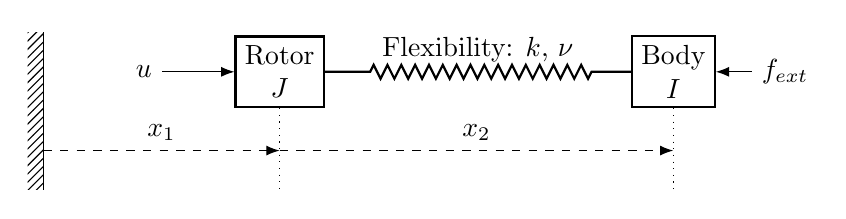
\begin{tikzpicture}[node distance = 5cm]
			\fill[pattern=north east lines, pattern color = black] (0,0.5) rectangle (-0.2,-1.5);
			\draw (0, 0.5) -- (0, -1.5);
			
			\node[draw, rectangle, thick, align=center] (rotor)  at (3, 0) {Rotor\\$J$};
			\node[draw, rectangle, thick, align=center, right of = rotor] (body) {Body\\$I$};
			
			\draw[dotted] (rotor) -- ++(0, -1.5);
			\draw[dotted] (body) -- ++(0, -1.5);
			\draw[dashed, -Latex] (0, -1) -- ($(rotor) + (0, -1)$) node[pos=0.5, above] {$x_1$};
			\draw[dashed, -Latex] ($(rotor) + (0, -1)$) -- ($(body) + (0, -1)$) node[pos=0.5, above] {$x_2$};
			
			\draw[Latex-] (rotor) -- ++(-1.5, 0) node[left] {$u$};
			\draw[Latex-] (body) -- ++(1, 0) node[right] {$f_{ext}$};
			\draw[thick,decorate,decoration={zigzag,pre length=0.5cm,post length=0.5cm,segment length=5}] (body) -- (rotor) node[pos = 0.5, above] {Flexibility: $k$, $\nu$};
		\end{tikzpicture}
		\caption{Representation of a flexible joint (prismatic): a spring-damper is placed between the rotor and the output body} \label{fig:SystemA}
	\end{subfigure}

	\begin{subfigure}{\textwidth}
		\centering
		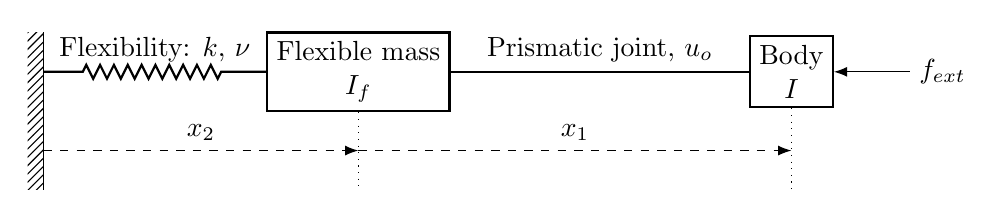
\begin{tikzpicture}[node distance = 5.5cm]
		\fill[pattern=north east lines, pattern color = black] (0,0.5) rectangle (-0.2,-1.5);
		\draw (0, 0.5) -- (0, -1.5);
		
		\node[draw, rectangle, thick, align=center] (rotor)  at (4, 0) {Flexible mass\\$I_f$};
		\node[draw, rectangle, thick, align=center, right of = rotor] (body) {Body\\$I$};
		
		\draw[dotted] (rotor) -- ++(0, -1.5);
		\draw[dotted] (body) -- ++(0, -1.5);
		\draw[dashed, -Latex] (0, -1) -- ($(rotor) + (0, -1)$) node[pos=0.5, above] {$x_2$};
		\draw[dashed, -Latex] ($(rotor) + (0, -1)$) -- ($(body) + (0, -1)$) node[pos=0.5, above] {$x_1$};
		
		\draw[Latex-] (body) -- ++(1.5, 0) node[right] {$f_{ext}$};
		\draw[thick,decorate,decoration={zigzag,pre length=0.5cm,post length=0.5cm,segment length=5}] (0, 0) -- (rotor) node[pos = 0.5, above] {Flexibility: $k$, $\nu$};
		\draw[thick] (rotor) -- (body) node[pos = 0.5, above] {Prismatic joint, $u_o$};
		\end{tikzpicture}
	\caption{The system actually being simulated by Jiminy: an extra mass is added to attach the spring. $u_o$ is the torque at the output of the transmission, and is equal to $u - J \ddot{x}_2$.} \label{fig:SystemB}
	\end{subfigure}
	\caption{A representation, for prismatic joints, of both systems under study.}
\end{figure}

However, such system cannot be easily represented in \emph{pinocchio}: indeed, \emph{pinocchio} implements rigid body dynamics as having a set of joints connecting rigid bodies: as such, it has no notion of transmission \emph{per se}. The rotor does not correspond to a physical part of inertia $J$ (the armature inertia, $J$, is computed for simple transmission by multiplying the real inertia by the square of the reduction ratio) - thus, rotor inertia is implemented in \emph{Jiminy} by modifying the corresponding diagonal term of the generalized inertia matrix (note that this approach works for simple, 1DoF joints, but is not generic). As such, it is no possible to add a degree of freedom to place the spring between the rotor and the output, as in the case in Figure~\ref{fig:SystemA}.

Instead, the flexibility is placed before rotor of the flexible joint being simulated. Since each joint must be connected to a body, this requires the addition of an extra body, connected to the flexibility: this body has its own inertia, $I_f$. In practice we will want $I_f$ close to zero, to avoid modifying the dynamical properties of the overall system. The resulting system is shown in Figure~\ref{fig:SystemB}

We now need to show that both systems are indeed equivalent, when taking the limit $I_f \rightarrow 0$. Consider the first, SEA system: applying Newton's law of motion to the rotor, then the output body, yields:
\begin{equation}
\left\{ 
\begin{aligned}
	J \ddot{x}_2 &= u + k x_1 + \nu \dot{x}_1 \\
	I (\ddot{x}_1 + \ddot{x}_2) &= -k x_1 -\nu \dot{x}_1 + f_{ext} \\
\end{aligned}
\right.
\end{equation}

which equivalently writes:
\begin{equation}
\left\{ 
\begin{aligned}
I (\ddot{x}_1 + \ddot{x}_2) &= -k x_1 -\nu \dot{x}_1 + f_{ext} \\
I (\ddot{x}_1 + \ddot{x}_2) + J \ddot{x}_2 &= u + f_{ext} \\
\end{aligned}
\right.
\label{eq:SystemA}
\end{equation}

The system simulated by Jiminy writes in turn:
\begin{equation}
\left\{ 
\begin{aligned}
I_f \ddot{x}_1 &= - k x_1 - \nu \dot{x}_1 - u_o\\
I (\ddot{x}_1 + \ddot{x}_2) &= u_o + f_{ext} \\
\end{aligned}
\right.
\label{eq:SystemB}
\end{equation}
 
where $u_o$ is the torque at the output of the transmission. Applying Euler's law to the rotor gives us: $J \ddot{x}_2 = u - u_o$. Thus, \eqref{eq:SystemB} rewrites:
\begin{equation}
\left\{ 
\begin{aligned}
I_f \ddot{x}_1 &= - k x_1 - \nu \dot{x}_1 - (u - J \ddot{x}_2)\\
I (\ddot{x}_1 + \ddot{x}_2)  &= u -J \ddot{x}_2 + f_{ext} \\
\end{aligned}
\right.
\end{equation}

add by adding both lines, we obtain:
\begin{equation}
\left\{ 
\begin{aligned}
(I + I_f) \ddot{x}_1 + I \ddot{x}_2 &= - k x_1 - \nu \dot{x}_1 + f_{ext}\\
I (\ddot{x}_1 + \ddot{x}_2) + J \ddot{x}_2 &= u + f_{ext} \\
\end{aligned}
\right.
\label{eq:SystemBPrime}
\end{equation}

Thus, from \eqref{eq:SystemA} and \eqref{eq:SystemBPrime}, it is now clear that both systems are equivalent when $I_f << I$. So while Jiminy does not exactly simulates a SEA as depicted in Figure~\ref{fig:SystemA}, it remains sufficiently close, in practice and for reasonable values of the output inertia $I$, to this system.

\end{document}